% Options for packages loaded elsewhere
\PassOptionsToPackage{unicode}{hyperref}
\PassOptionsToPackage{hyphens}{url}
\PassOptionsToPackage{dvipsnames,svgnames,x11names}{xcolor}
%
\documentclass[
  a4paper,
  DIV=11,
  numbers=noendperiod,
  oneside]{scrartcl}

\usepackage{amsmath,amssymb}
\usepackage{lmodern}
\usepackage{iftex}
\ifPDFTeX
  \usepackage[T1]{fontenc}
  \usepackage[utf8]{inputenc}
  \usepackage{textcomp} % provide euro and other symbols
\else % if luatex or xetex
  \usepackage{unicode-math}
  \defaultfontfeatures{Scale=MatchLowercase}
  \defaultfontfeatures[\rmfamily]{Ligatures=TeX,Scale=1}
\fi
% Use upquote if available, for straight quotes in verbatim environments
\IfFileExists{upquote.sty}{\usepackage{upquote}}{}
\IfFileExists{microtype.sty}{% use microtype if available
  \usepackage[]{microtype}
  \UseMicrotypeSet[protrusion]{basicmath} % disable protrusion for tt fonts
}{}
\makeatletter
\@ifundefined{KOMAClassName}{% if non-KOMA class
  \IfFileExists{parskip.sty}{%
    \usepackage{parskip}
  }{% else
    \setlength{\parindent}{0pt}
    \setlength{\parskip}{6pt plus 2pt minus 1pt}}
}{% if KOMA class
  \KOMAoptions{parskip=half}}
\makeatother
\usepackage{xcolor}
\usepackage[left=1in,marginparwidth=2.0in,textwidth=4.0in,marginparsep=0.3in]{geometry}
\setlength{\emergencystretch}{3em} % prevent overfull lines
\setcounter{secnumdepth}{5}
% Make \paragraph and \subparagraph free-standing
\ifx\paragraph\undefined\else
  \let\oldparagraph\paragraph
  \renewcommand{\paragraph}[1]{\oldparagraph{#1}\mbox{}}
\fi
\ifx\subparagraph\undefined\else
  \let\oldsubparagraph\subparagraph
  \renewcommand{\subparagraph}[1]{\oldsubparagraph{#1}\mbox{}}
\fi


\providecommand{\tightlist}{%
  \setlength{\itemsep}{0pt}\setlength{\parskip}{0pt}}\usepackage{longtable,booktabs,array}
\usepackage{calc} % for calculating minipage widths
% Correct order of tables after \paragraph or \subparagraph
\usepackage{etoolbox}
\makeatletter
\patchcmd\longtable{\par}{\if@noskipsec\mbox{}\fi\par}{}{}
\makeatother
% Allow footnotes in longtable head/foot
\IfFileExists{footnotehyper.sty}{\usepackage{footnotehyper}}{\usepackage{footnote}}
\makesavenoteenv{longtable}
\usepackage{graphicx}
\makeatletter
\def\maxwidth{\ifdim\Gin@nat@width>\linewidth\linewidth\else\Gin@nat@width\fi}
\def\maxheight{\ifdim\Gin@nat@height>\textheight\textheight\else\Gin@nat@height\fi}
\makeatother
% Scale images if necessary, so that they will not overflow the page
% margins by default, and it is still possible to overwrite the defaults
% using explicit options in \includegraphics[width, height, ...]{}
\setkeys{Gin}{width=\maxwidth,height=\maxheight,keepaspectratio}
% Set default figure placement to htbp
\makeatletter
\def\fps@figure{htbp}
\makeatother
\newlength{\cslhangindent}
\setlength{\cslhangindent}{1.5em}
\newlength{\csllabelwidth}
\setlength{\csllabelwidth}{3em}
\newlength{\cslentryspacingunit} % times entry-spacing
\setlength{\cslentryspacingunit}{\parskip}
\newenvironment{CSLReferences}[2] % #1 hanging-ident, #2 entry spacing
 {% don't indent paragraphs
  \setlength{\parindent}{0pt}
  % turn on hanging indent if param 1 is 1
  \ifodd #1
  \let\oldpar\par
  \def\par{\hangindent=\cslhangindent\oldpar}
  \fi
  % set entry spacing
  \setlength{\parskip}{#2\cslentryspacingunit}
 }%
 {}
\usepackage{calc}
\newcommand{\CSLBlock}[1]{#1\hfill\break}
\newcommand{\CSLLeftMargin}[1]{\parbox[t]{\csllabelwidth}{#1}}
\newcommand{\CSLRightInline}[1]{\parbox[t]{\linewidth - \csllabelwidth}{#1}\break}
\newcommand{\CSLIndent}[1]{\hspace{\cslhangindent}#1}

\KOMAoption{captions}{tableheading}
\makeatletter
\makeatother
\makeatletter
\makeatother
\makeatletter
\@ifpackageloaded{caption}{}{\usepackage{caption}}
\AtBeginDocument{%
\ifdefined\contentsname
  \renewcommand*\contentsname{Table of contents}
\else
  \newcommand\contentsname{Table of contents}
\fi
\ifdefined\listfigurename
  \renewcommand*\listfigurename{List of Figures}
\else
  \newcommand\listfigurename{List of Figures}
\fi
\ifdefined\listtablename
  \renewcommand*\listtablename{List of Tables}
\else
  \newcommand\listtablename{List of Tables}
\fi
\ifdefined\figurename
  \renewcommand*\figurename{Figure}
\else
  \newcommand\figurename{Figure}
\fi
\ifdefined\tablename
  \renewcommand*\tablename{Table}
\else
  \newcommand\tablename{Table}
\fi
}
\@ifpackageloaded{float}{}{\usepackage{float}}
\floatstyle{ruled}
\@ifundefined{c@chapter}{\newfloat{codelisting}{h}{lop}}{\newfloat{codelisting}{h}{lop}[chapter]}
\floatname{codelisting}{Listing}
\newcommand*\listoflistings{\listof{codelisting}{List of Listings}}
\makeatother
\makeatletter
\@ifpackageloaded{caption}{}{\usepackage{caption}}
\@ifpackageloaded{subcaption}{}{\usepackage{subcaption}}
\makeatother
\makeatletter
\@ifpackageloaded{tcolorbox}{}{\usepackage[many]{tcolorbox}}
\makeatother
\makeatletter
\@ifundefined{shadecolor}{\definecolor{shadecolor}{rgb}{.97, .97, .97}}
\makeatother
\makeatletter
\@ifpackageloaded{sidenotes}{}{\usepackage{sidenotes}}
\@ifpackageloaded{marginnote}{}{\usepackage{marginnote}}
\makeatother
\makeatletter
\makeatother
\ifLuaTeX
  \usepackage{selnolig}  % disable illegal ligatures
\fi
\IfFileExists{bookmark.sty}{\usepackage{bookmark}}{\usepackage{hyperref}}
\IfFileExists{xurl.sty}{\usepackage{xurl}}{} % add URL line breaks if available
\urlstyle{same} % disable monospaced font for URLs
\hypersetup{
  pdftitle={Translating priors from linear mixed models to repeated-measures ANOVA and paired t tests},
  pdfauthor={Frederik Aust \& Julia Haaf},
  colorlinks=true,
  linkcolor={blue},
  filecolor={Maroon},
  citecolor={Blue},
  urlcolor={Blue},
  pdfcreator={LaTeX via pandoc}}

\title{Translating priors from linear mixed models to repeated-measures
ANOVA and paired \(t\) tests}
\usepackage{etoolbox}
\makeatletter
\providecommand{\subtitle}[1]{% add subtitle to \maketitle
  \apptocmd{\@title}{\par {\large #1 \par}}{}{}
}
\makeatother
\subtitle{Supplement to \emph{Bayes Factors for Mixed Models:
Perspective on Responses}}
\author{Frederik Aust \& Julia Haaf}
\date{2022-09-27}

\begin{document}
\maketitle
\ifdefined\Shaded\renewenvironment{Shaded}{\begin{tcolorbox}[interior hidden, borderline west={3pt}{0pt}{shadecolor}, sharp corners, enhanced, frame hidden, boxrule=0pt, breakable]}{\end{tcolorbox}}\fi

\renewcommand*\contentsname{Table of contents}
{
\hypersetup{linkcolor=}
\setcounter{tocdepth}{3}
\tableofcontents
}
In van Doorn et al. (2021), we give Example 1 in which Bayes factors in
mixed models with standardized effect size parameterization (Rouder et
al. 2012) change when error variance decreases. We assumed a simple
repeated-measures design with \(I\) participants responding \(K\) times
in each of two conditions. The maximal model for these data is our Model
6 with random intercepts \(\alpha_i\) and random slopes \(\theta_i\),

\[
\begin{aligned}
y_{ijk} & \sim \mathcal{N}(\mu + \sigma_\epsilon (\alpha_i + x_j (\nu + \theta_i)), \sigma^2_\epsilon) \\ & \\
\alpha_i & \sim \mathcal{N}(0, g_\alpha) \\
\nu & \sim \mathcal{N}(0, g_{\nu}) \\
\theta_i & \sim \mathcal{N}(0, g_\theta) \\ & \\
g_{\alpha} & \sim \mathcal{IG}(0.5, 0.5~r_{\alpha}^2) \\
g_{\nu} & \sim \mathcal{IG}(0.5, 0.5~r_{\nu}^2) \\
g_{\theta} & \sim \mathcal{IG}(0.5, 0.5~r_{\theta}^2) \\ & \\
(\mu, \sigma^2_\epsilon) & = 1/\sigma^2_\epsilon.
\end{aligned}
\]

\hypertarget{reduced-error-variance-through-aggregation}{%
\section{Reduced error variance through
aggregation}\label{reduced-error-variance-through-aggregation}}

Because priors are placed on standardized effect sizes, a reduction of
\(\sigma_\epsilon\) increases prior plausibility of larger effect sizes.
In our Example 1, measurement error decreases as the number of
aggregated trials \(n\) increases,
\(\sigma\prime_\epsilon = \frac{\sigma_\epsilon}{\sqrt{n}}\),

\[
\begin{aligned}
y_{ijk} & \sim \mathcal{N}(\mu + \sigma\prime_\epsilon (\alpha_i + x_j (\nu + \theta_i)), \sigma\prime_\epsilon^{2}) \\ & \\
\alpha_i & \sim \mathcal{N}(0, g_\alpha) \\
\nu & \sim \mathcal{N}(0, g_\theta) \\
\theta_i & \sim \mathcal{N}(0, g_\theta).
\end{aligned}
\]

This further implies the priors

\[
\begin{aligned}
\nu & \sim \mathcal{N}(0, g_{\nu}/\sqrt{n}) \\
g_\alpha & \sim \mathcal{IG}(0.5, 0.5~r^2_{\alpha}/\sqrt{n}) \\
g_\theta & \sim\mathcal{IG}(0.5, 0.5~r^2_{\theta}/\sqrt{n}).
\end{aligned}
\]

Hence, to obtain equivalent Bayes factors the prior scales should be
adjusted accordingly, \(r\prime^2 = r^2 \sqrt{n}\).

\hypertarget{simulation}{%
\subsection{Simulation}\label{simulation}}

To test whether this prior adjustment works as intended across all
levels of aggregation, we conducted a small simulation for the balanced
null comparison. We simulated \(K = 100\) trials for \(I = 20\)
participants (\(\mu = 1\); \(\sigma_\alpha = 0.5\);
\(\nu = \{0, 0.2, 0.4\}\); \(\sigma_\theta = \{0.1, 0.25, 0.5, 1, 2\}\);
\(\sigma_\epsilon = 1\)). As in our Example 1, the data were generated
deterministically with identical condition and participant means as well
as standard errors across all levels of aggregation (\(n\)).

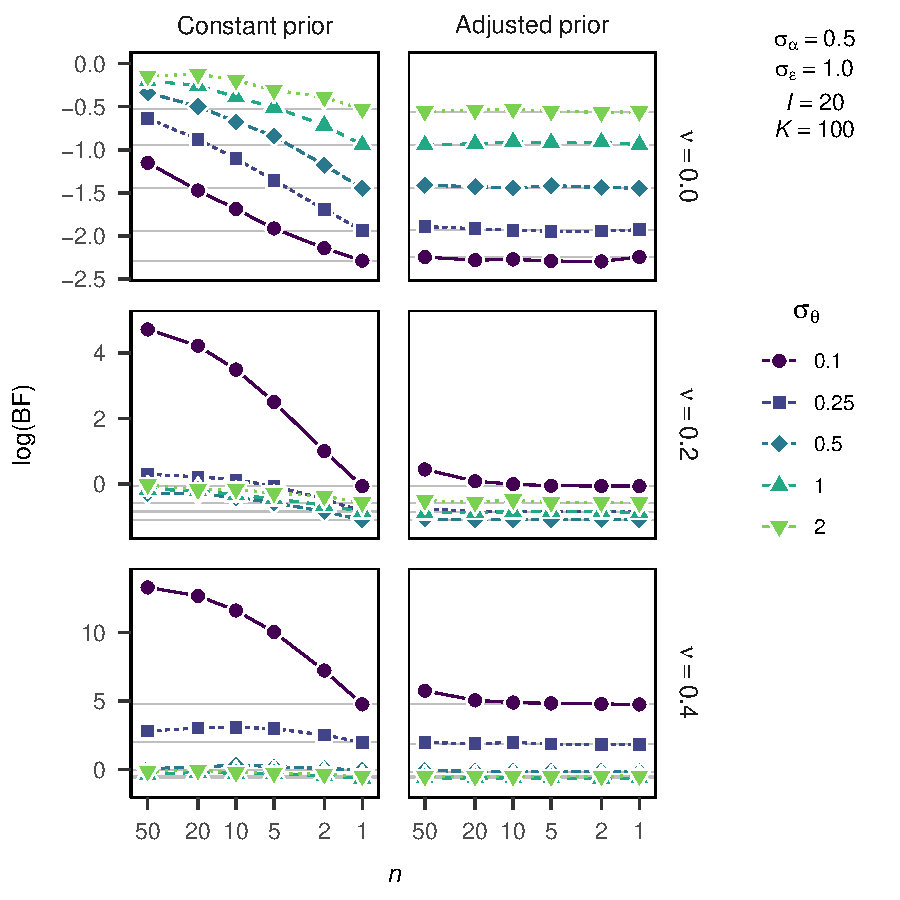
\includegraphics{prior_translation_files/figure-pdf/unnamed-chunk-3-1.pdf}

Horizontal lines represent \(\log{\mathrm{BF}}\) for each level of
\(\sigma_\theta\) with \(n = 1\) (no aggregation) as reference. The
results confirm that the prior adjustment works well. Only when an
effect is present and the random slope variance \(\sigma_\theta^2\) is
small, we observed a minor inflation of the Bayes factor for \(n = 50\).
This bias scaled with \(\log{BF}\) and was negligible for small and
inconsequential for large Bayes factors.

\hypertarget{full-aggregation}{%
\section{Full aggregation}\label{full-aggregation}}

When aggregating each participant's data to a single observation per
cell the data can analyzed in two ways: By modeling participants' (1)
cell means using a one-way repeated-measures ANOVA, or (2) cell mean
differences using a paired \(t\)-test.

\hypertarget{repeated-measures-anova}{%
\subsection{Repeated-measures ANOVA}\label{repeated-measures-anova}}

When data are fully aggregated data (i.e., \(n = K\)), the random slopes
variance \(\sigma_\theta^2\) folds into the error variance
\(\sigma_\epsilon^2\). That is, Model 6 reduces to Model 4,

\[
\begin{aligned}
\bar{y}_{ij\cdot} & \sim \mathcal{N}(\mu + \sigma\prime_\epsilon (\alpha_i + x_j \nu), \sigma\prime_\epsilon^2 + \sigma_\theta^2/2) \\
\alpha_i & \sim \mathcal{N}(0, g_\alpha \sqrt{\sigma_\theta^2}) \\
\nu & \sim \mathcal{N}(0, g_{\nu} \sqrt{\sigma_\theta^2/2}).
\end{aligned}
\]

The random slopes variance \(\sigma_\theta^2\) is scaled by the
orthonormal effect coding, \(\pm \sqrt{2}/2\). Compared to partial
aggregation, the adjustment for the fixed effect requires an additional
factor that depends on a weighted ratio of random variance
\(\sigma^2_\theta\) and error variance \(\sigma^2_\epsilon\),

\[
\begin{aligned}
\sqrt{\sigma_\epsilon^2/K + \sigma_\theta^2/2} & = \sigma_\epsilon/\sqrt{K} \sqrt{1 + \frac{K\sigma^2_\theta}{2\sigma_\epsilon^2}} \\
  & = \sigma_\epsilon/\sqrt{K} \sqrt{\frac{2\sigma_\epsilon^2 + K\sigma^2_\theta}{2\sigma_\epsilon^2}} \\
  & = \sigma_\epsilon/\sqrt{K} \sqrt{\frac{2/K + \sigma^2_\theta/\sigma_\epsilon^2}{2/K}} \\
\end{aligned}
\]

For random intercepts, the additional correction factor is obtained by
marginalizing over the dummy coded random effect, yielding a weight of 1
for the random slope variance.

\hypertarget{t-test}{%
\subsection{\texorpdfstring{\(t\) Test}{t Test}}\label{t-test}}

For the paired \(t\)-test the prior adjustment additionally must account
for the different model parameterization (\(\pm 0.5\)
vs.~\(\pm \sqrt{2}/2\)),

\[
\begin{aligned}
\bar{y}_{ij\cdot} - \bar{y}_{ij\cdot} & \sim \mathcal{N}(\mu + \sigma\prime_\epsilon (\alpha_i + 0.5 \nu), \sigma\prime_\epsilon^2) \\
& - \mathcal{N}(\mu + \sigma\prime_\epsilon (\alpha_i - 0.5 \nu), \sigma\prime_\epsilon^2) \\
  & = \mathcal{N}(\sigma\prime_\epsilon \nu, 2\sigma\prime_\epsilon^2) \\ & \\
\end{aligned}
\]

Rescaling the prior on \(\nu\) to the orthonormal scale,
\(\sqrt{2}\nu\), yields the same adjustment as for the ANOVA prior,

\[
\begin{aligned}
\sqrt{\sigma_\epsilon^2/K + \sigma_\theta^2/2} & = \sigma_\epsilon/\sqrt{K} \sqrt{1 + \frac{K\sigma^2_\theta}{2\sigma_\epsilon^2}} \\
  & = \sigma_\epsilon/\sqrt{K} \sqrt{\frac{2\sigma_\epsilon^2 + K\sigma^2_\theta}{2\sigma_\epsilon^2}} \\
  & = \sigma_\epsilon/\sqrt{K} \sqrt{\frac{2/K + \sigma^2_\theta/\sigma_\epsilon^2}{2/K}}. \\
\end{aligned}
\]

Note that in the linear mixed model \(\sigma_\theta^2\) is characterized
by a probability distribution, which prohibits a translation of the
prior in terms of an adjusted scaling factor. To test whether the
adjustment can be approximated by using a point estimate, we conducted a
simulation for balanced null comparisons.

\hypertarget{simulation-1}{%
\subsection{Simulation}\label{simulation-1}}

We randomly simulated \(K = \{5, 25, 100\}\) responses for
\(I = \{20, 50, 100, 200\}\) participants (\(\mu = 1\);
\(\sigma_\alpha = 0.5\); \(\nu = \{0, 0.2, 0.5\}\);
\(\sigma_\theta = 0.5\); \(\sigma_\epsilon = \{0.1, 0.25, 0.5, 1, 2\}\))
10 times each.

\hypertarget{mixed-model-vs.-t-test}{%
\paragraph{Mixed model vs.~t-test}\label{mixed-model-vs.-t-test}}

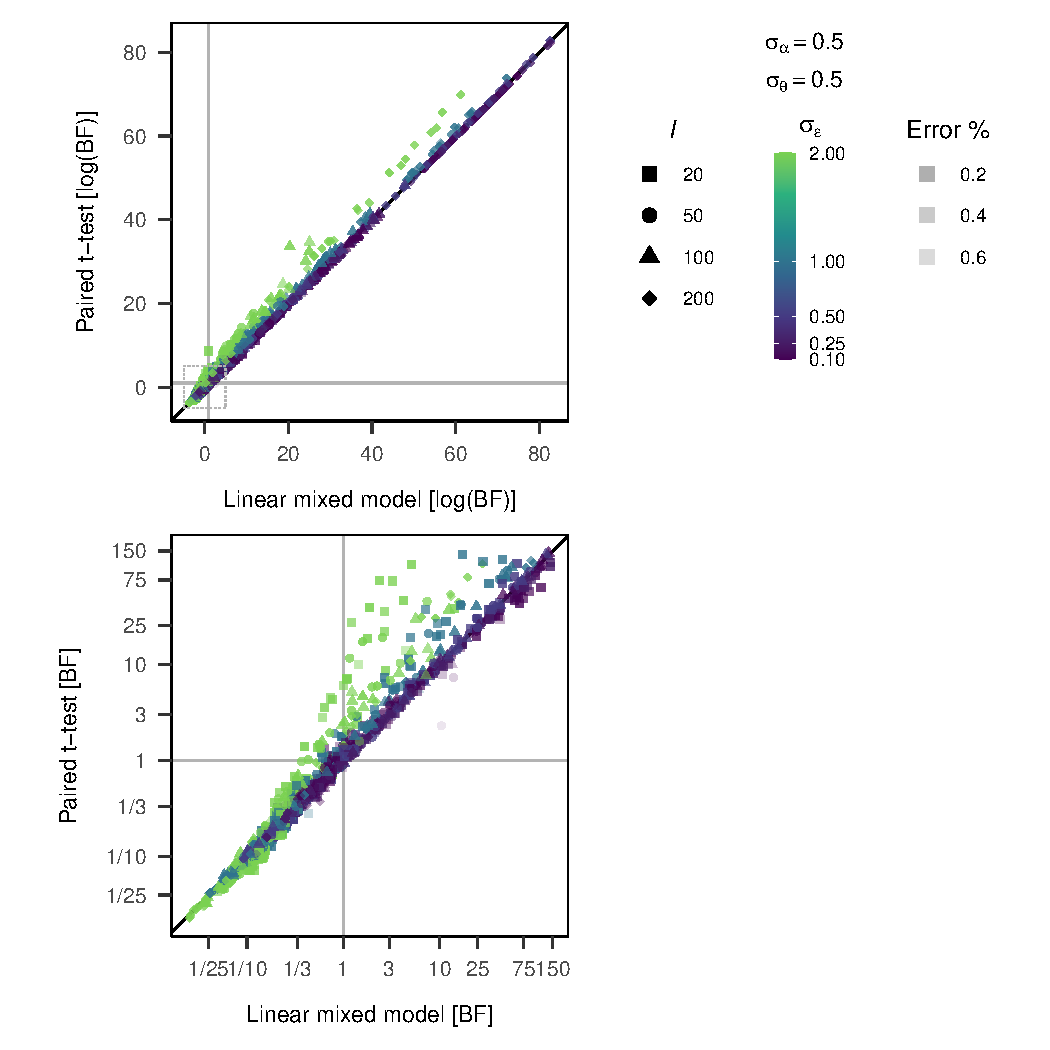
\includegraphics{prior_translation_files/figure-pdf/simulation-results1-1.pdf}

Results split by all varied factors

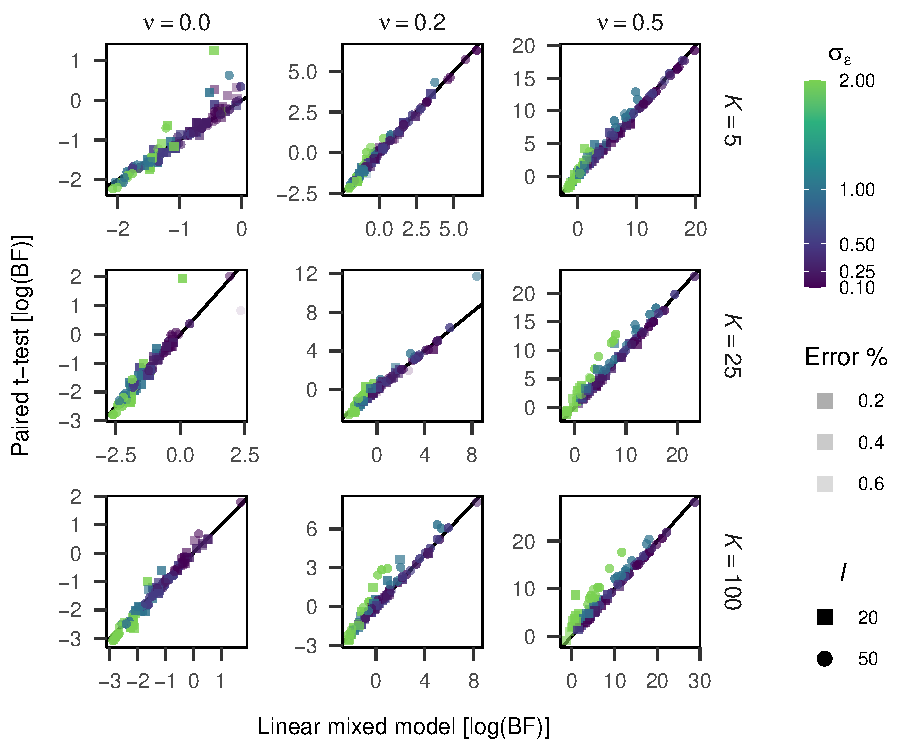
\includegraphics{prior_translation_files/figure-pdf/simulation-results1-details-1.pdf}

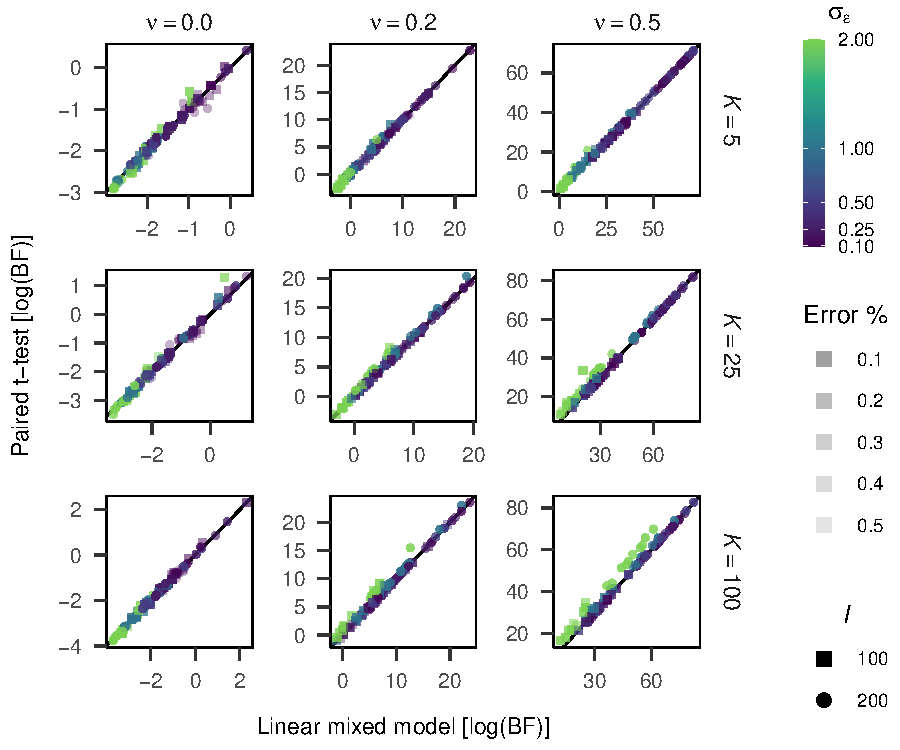
\includegraphics{prior_translation_files/figure-pdf/simulation-results1-details-2.pdf}

\hypertarget{mixed-model-vs.-rm-anova}{%
\paragraph{Mixed model vs.~RM-ANOVA}\label{mixed-model-vs.-rm-anova}}

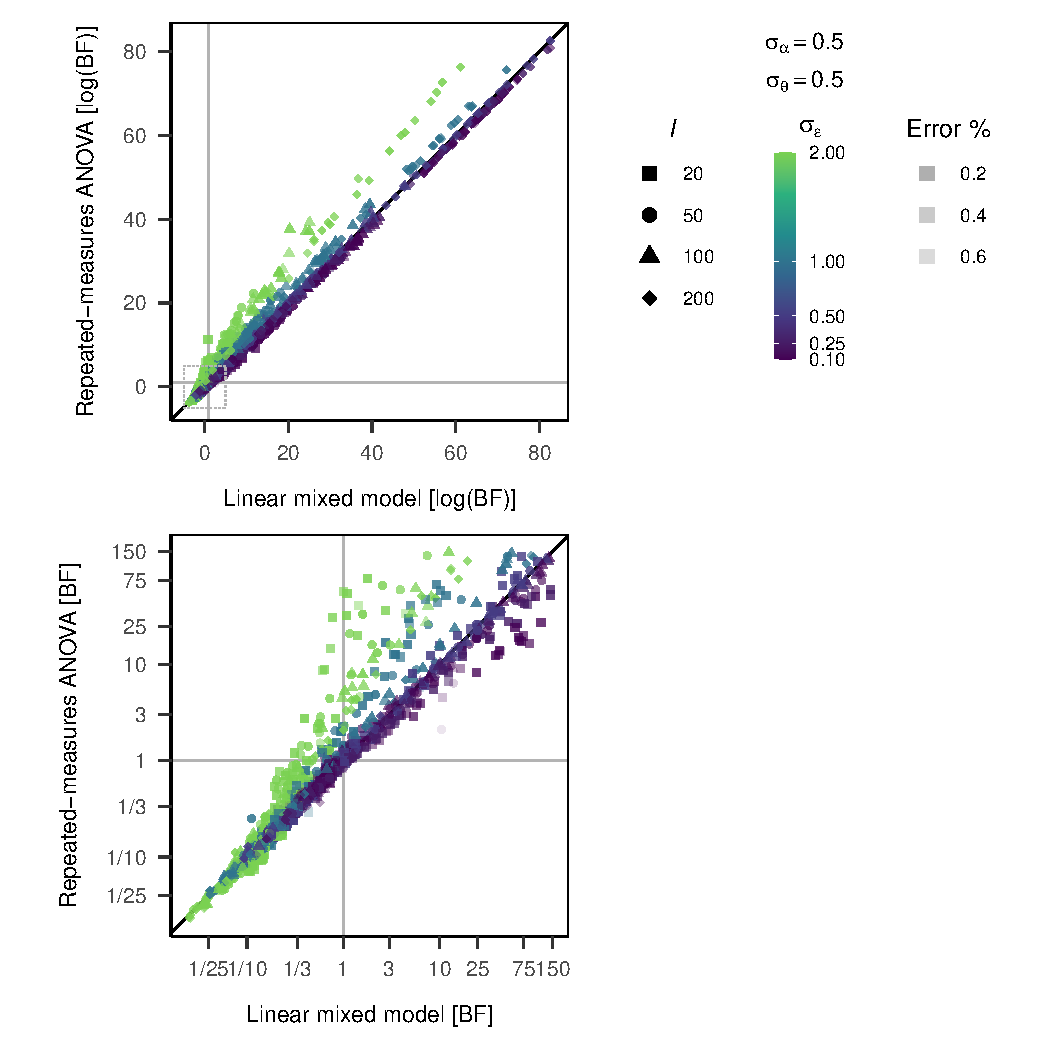
\includegraphics{prior_translation_files/figure-pdf/simulation-results2-1.pdf}

Results split by all varied factors

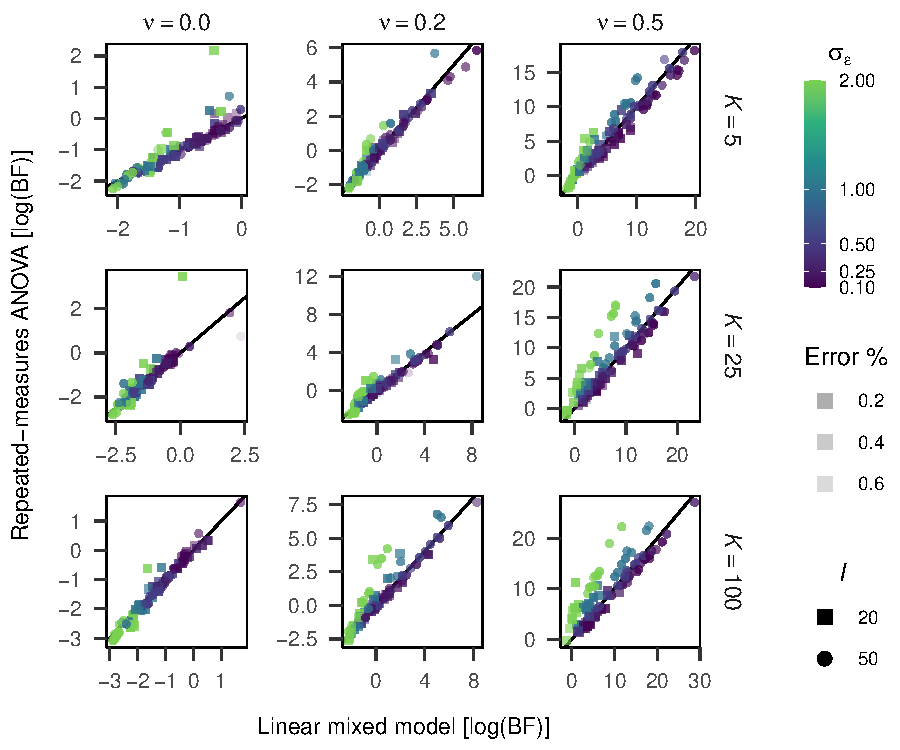
\includegraphics{prior_translation_files/figure-pdf/simulation-results2-details-1.pdf}

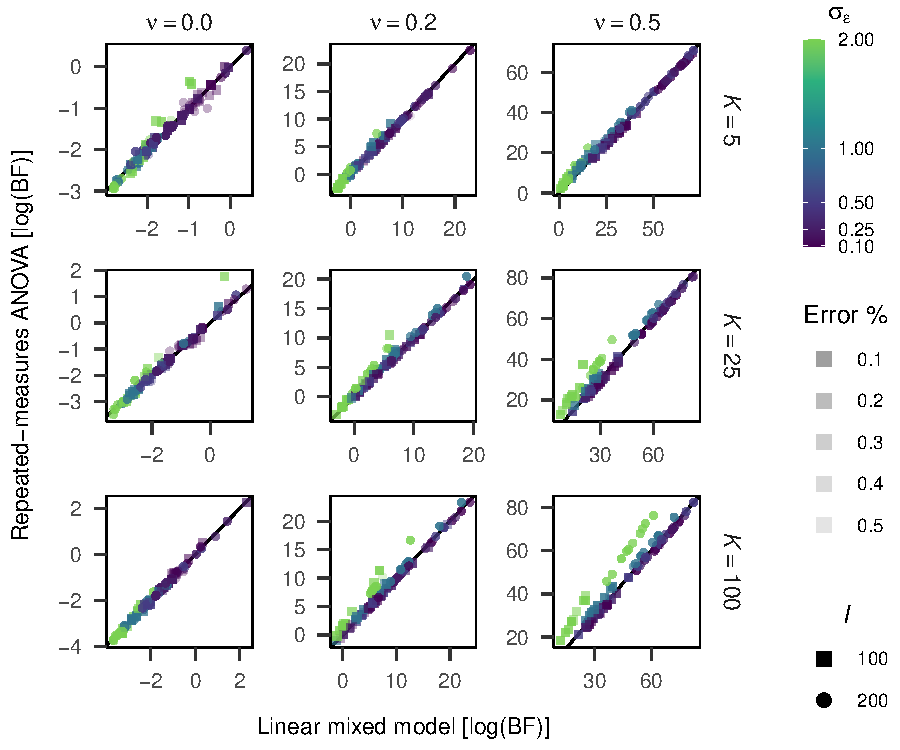
\includegraphics{prior_translation_files/figure-pdf/simulation-results2-details-2.pdf}

\hypertarget{rm-anova-vs.-t-test}{%
\paragraph{RM-ANOVA vs.~t-test}\label{rm-anova-vs.-t-test}}

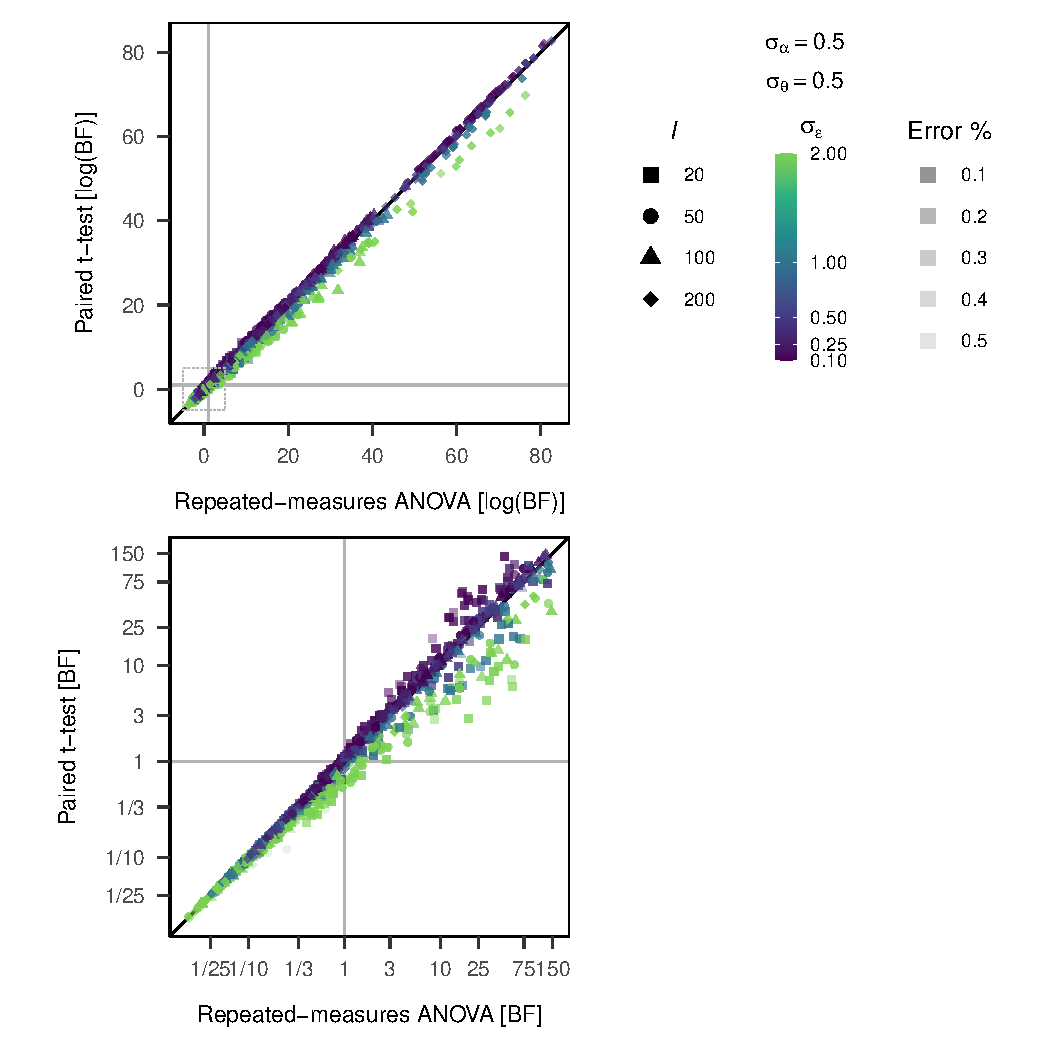
\includegraphics{prior_translation_files/figure-pdf/simulation-results3-1.pdf}

Results split by all varied factors

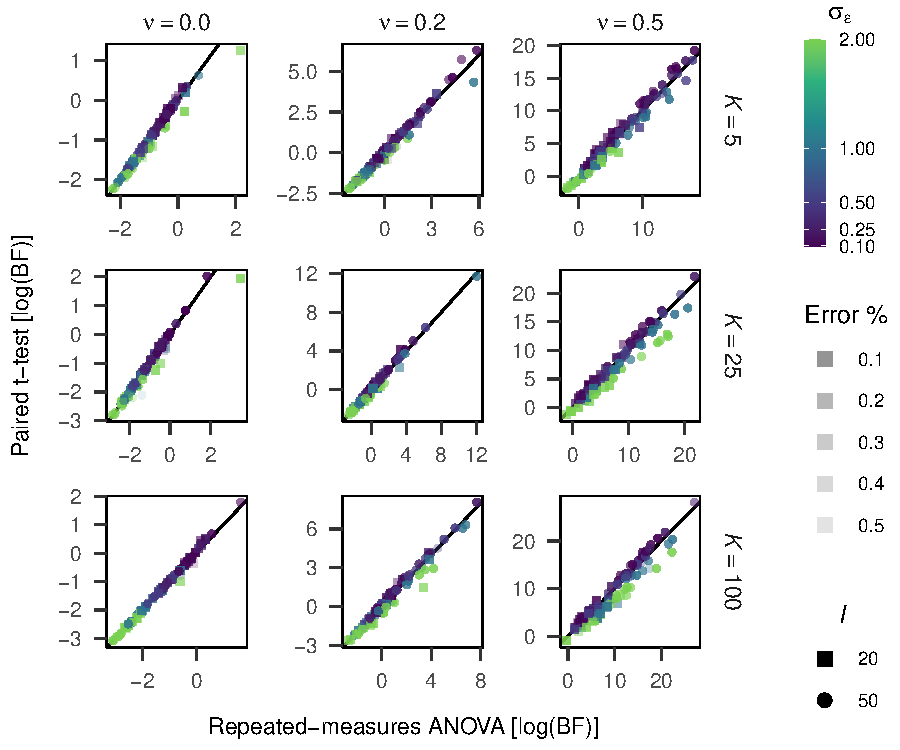
\includegraphics{prior_translation_files/figure-pdf/simulation-results3-details-1.pdf}

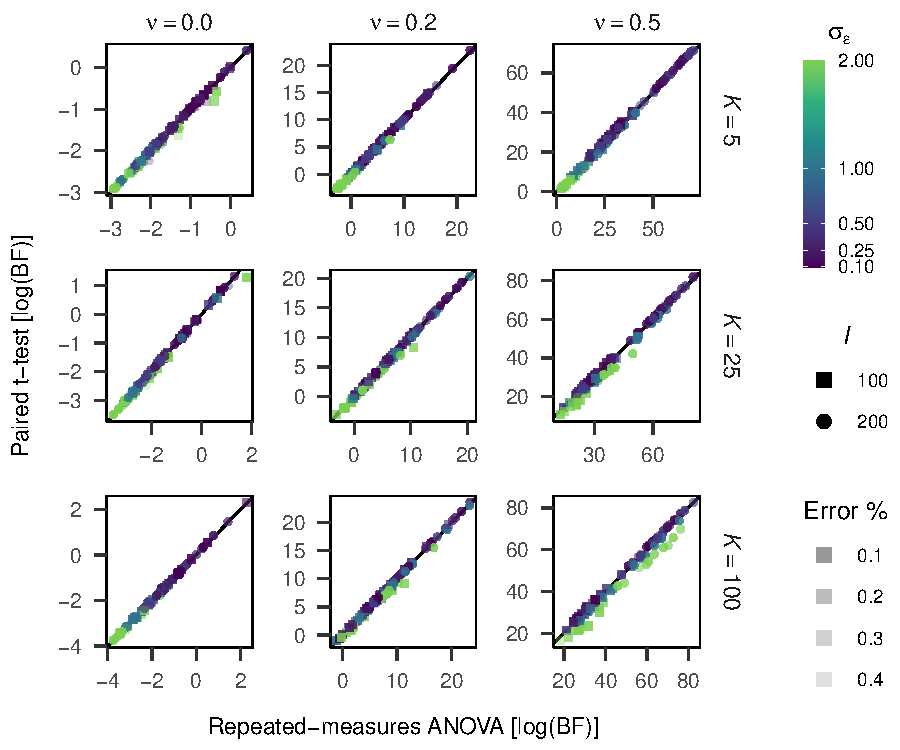
\includegraphics{prior_translation_files/figure-pdf/simulation-results3-details-2.pdf}

When the error variance \(\sigma_\epsilon^2\) is small or the sample
size \(I\) is large, the adjustments works well. However, compared to
the linear mixed model, both aggregate analyses produced diverging Bayes
factors. As illustrated by the following trend lines, the divergence
increased as (1) the difference in random slope and error variance
increased and (2) the number of participants decreased. The divergence
of Bayes factors was more pronounced in the repeated-measures ANOVA than
in the paired \(t\)-test, because priors on both fixed and random
effects require adjustment.

\hypertarget{mixed-model-vs.-t-test-1}{%
\paragraph{Mixed model vs.~t-test}\label{mixed-model-vs.-t-test-1}}

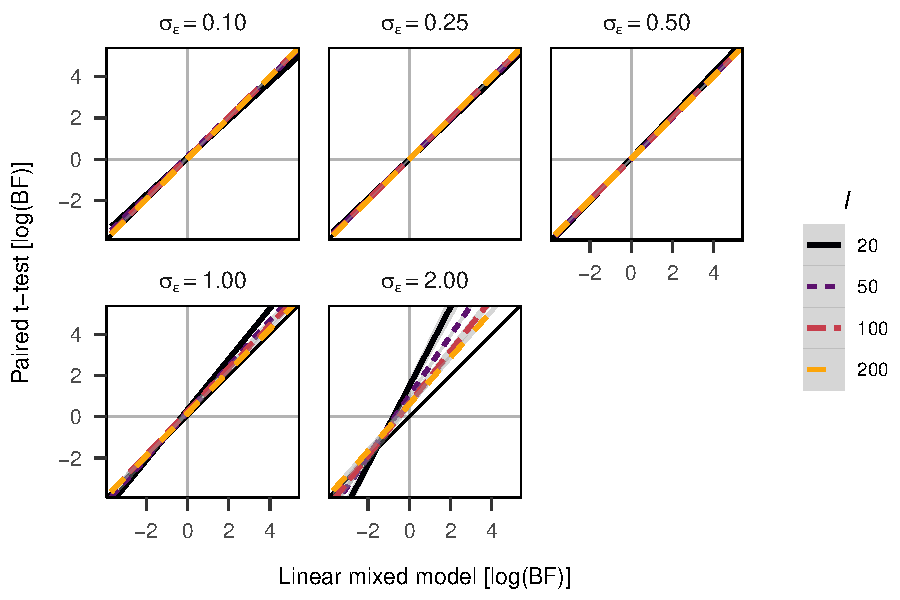
\includegraphics{prior_translation_files/figure-pdf/trend-plots-ttest-1.pdf}

Intercepts and slopes as a function of \(I\) and \(\sigma_\epsilon\)

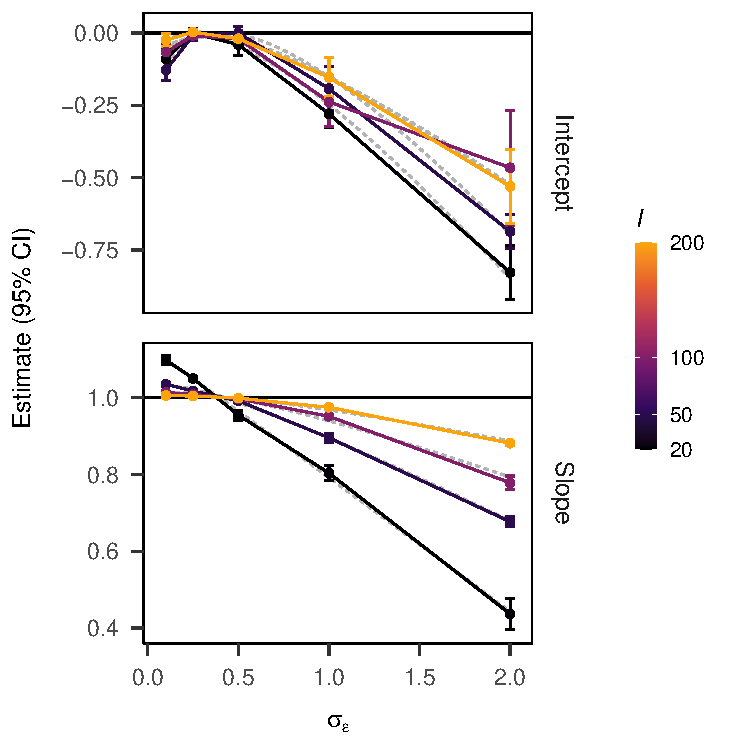
\includegraphics{prior_translation_files/figure-pdf/trend-plots-ttest-exploration-1.pdf}

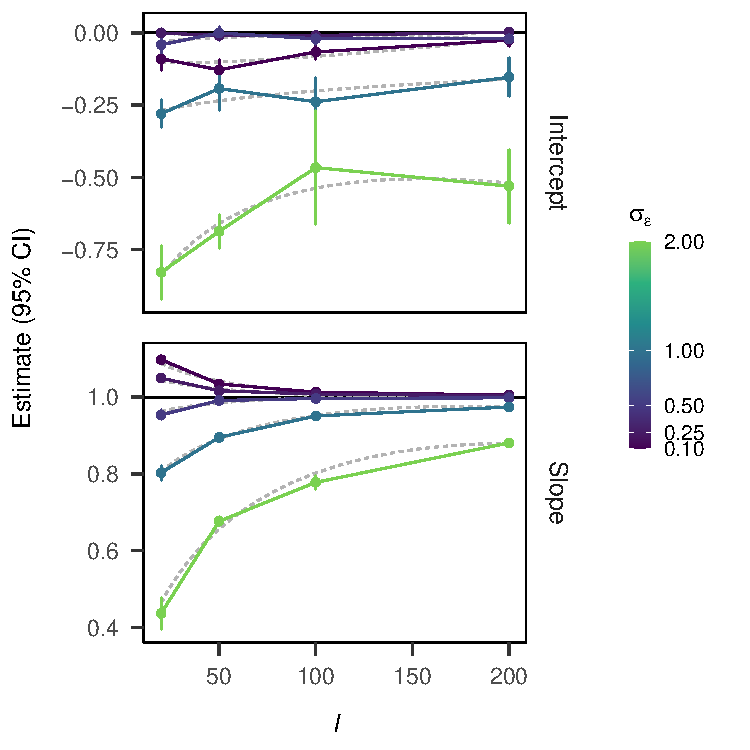
\includegraphics{prior_translation_files/figure-pdf/trend-plots-ttest-exploration-2.pdf}

\hypertarget{mixed-model-vs.-rm-anova-1}{%
\paragraph{Mixed model vs.~RM-ANOVA}\label{mixed-model-vs.-rm-anova-1}}

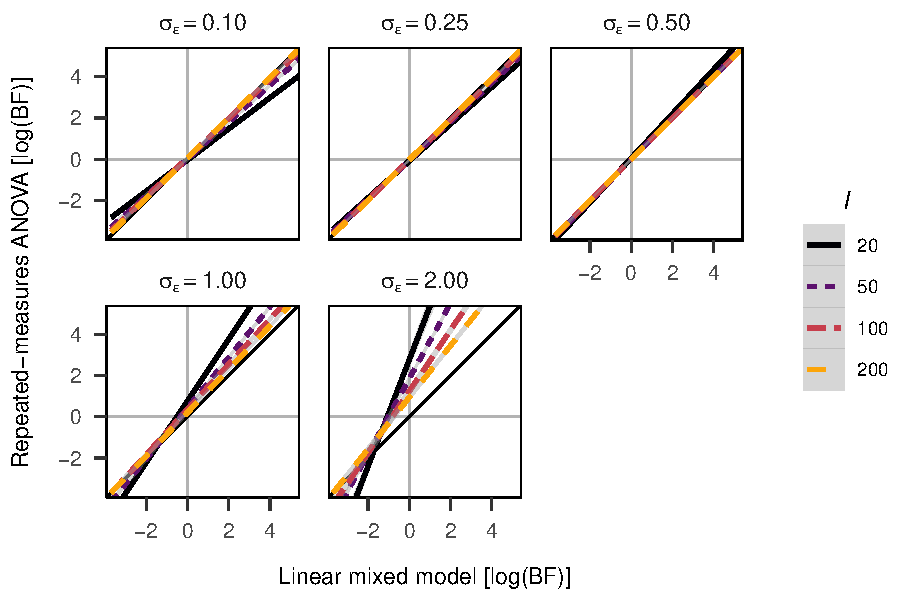
\includegraphics{prior_translation_files/figure-pdf/trend-plots-anova-1.pdf}

Intercepts and slopes as a function of \(I\) and \(\sigma_\epsilon\)

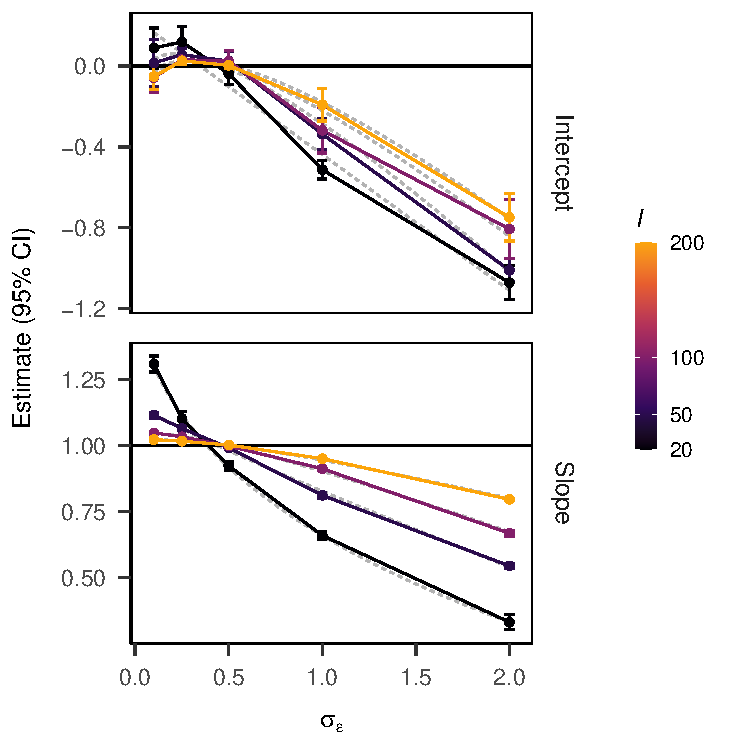
\includegraphics{prior_translation_files/figure-pdf/trend-plots-anova-exploration-1.pdf}

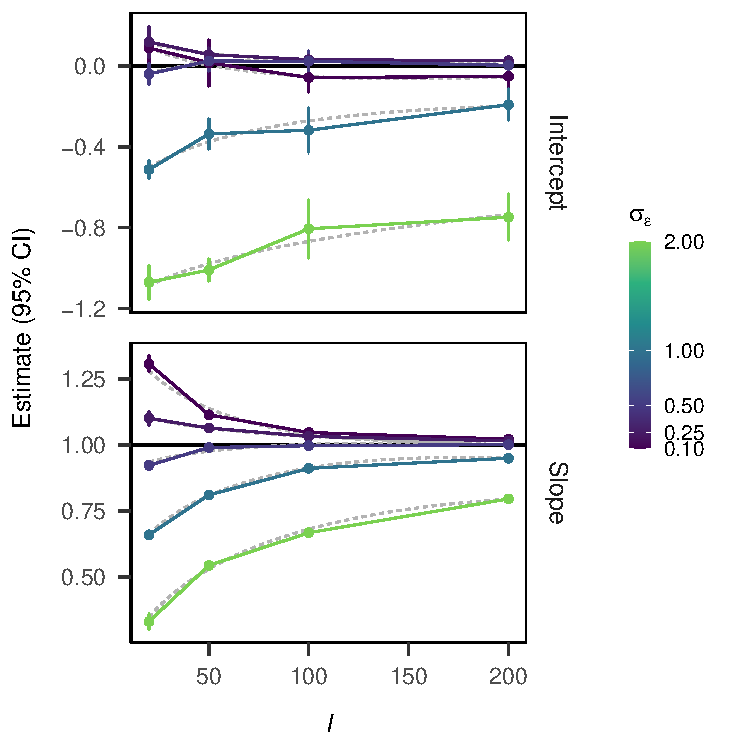
\includegraphics{prior_translation_files/figure-pdf/trend-plots-anova-exploration-2.pdf}

We examined how intercepts and slopes of the trend lines varied with
error variance and number of participants. Using AIC and BIC, we
compared several regression models that expressed the Bayes factors from
the full mixed model (weighted by the reciprocal of their estimation
error) as a function of Bayes factors from the corresponding paired
\(t\)-test, sample size \(I\), and error variance \(\sigma_\epsilon^2\).
We compared the same set of models for the Bayes factors from
repeated-measures ANOVA and found the same winning model. The Bayes
factors predicted by the selected model,

\[
\begin{aligned}
\log\mathrm{BF_{LMM}} = & ~ b_1 \sigma_\epsilon + b_2 \sqrt{\sigma_\epsilon} + b_3 \sqrt{I} + b_4 \sqrt{I} \sigma_\epsilon +\\
    & ~\log \mathrm{BF} (1 + b_5 \sigma_\epsilon^2 + b_6 \log I + b_7 \sigma_\epsilon^2 \log I),
\end{aligned}
\]

largely offset divergences between linear mixed model and aggregate
analyses.

\hypertarget{mixed-model-vs.-t-test-2}{%
\paragraph{Mixed model vs.~t-test}\label{mixed-model-vs.-t-test-2}}

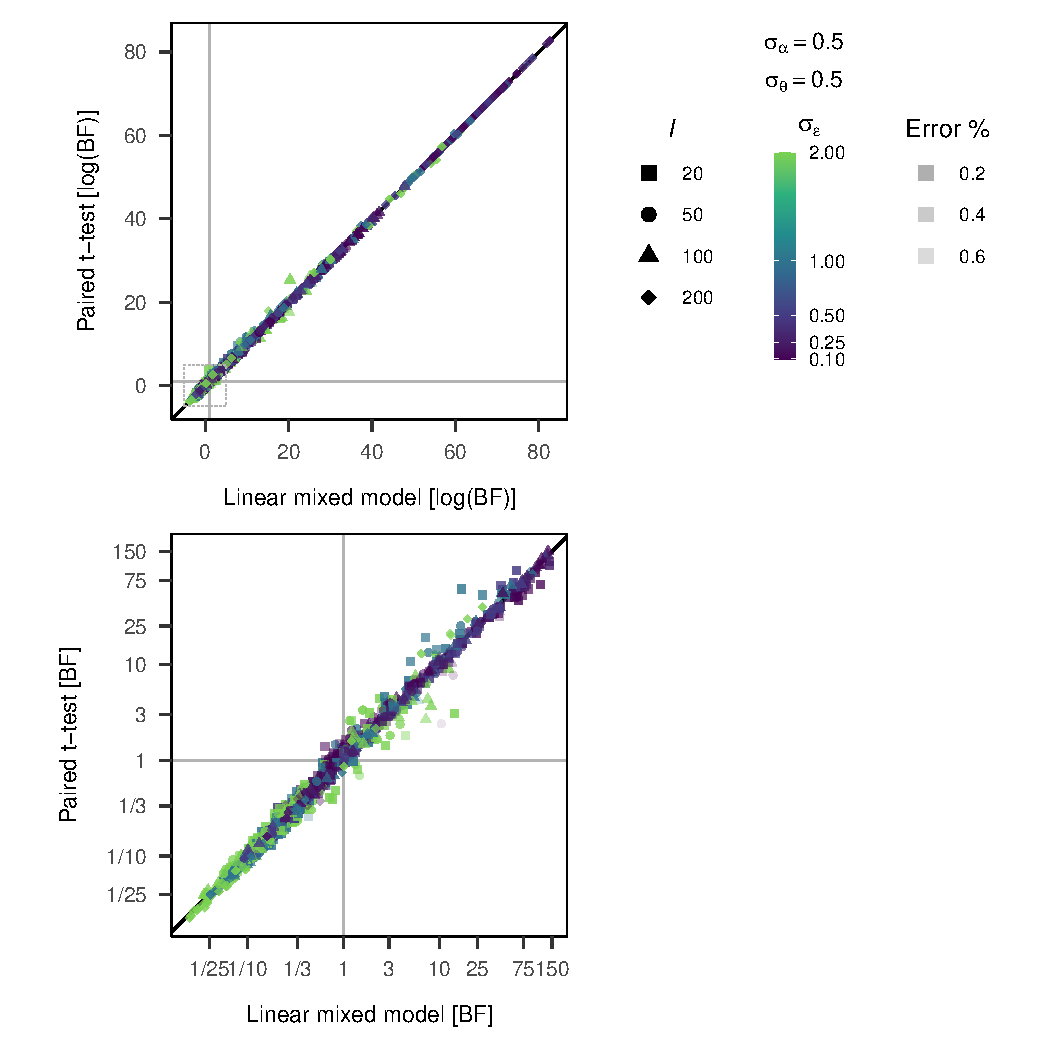
\includegraphics{prior_translation_files/figure-pdf/bias-correction-ttest-1.pdf}

Estimated regression coefficients

(\#tab:bias-correction-ttest-coef)

\emph{Results for regression of \(\log \mathrm{BF}\) from linear mixed
models on \(\log \mathrm{BF}\) from paired t-tests.}

\begin{longtable}[]{@{}lrcrr@{}}
\toprule()
Predictor & \(b\) & 95\% CI & \(t(1793)\) & \(p\) \\
\midrule()
\endhead
\(\sigma_\epsilon\) & -0.835 & {[}-0.949, -0.721{]} & -14.32 &
\textless{} .001 \\
\(\sqrt{\sigma_\epsilon}\) & 0.551 & {[}0.419, 0.684{]} & 8.16 &
\textless{} .001 \\
\(\sqrt{I}\) & -0.009 & {[}-0.015, -0.003{]} & -2.89 & .004 \\
\(\sigma_\epsilon\) \(\times\) \(\sqrt{I}\) & 0.019 & {[}0.013, 0.025{]}
& 6.35 & \textless{} .001 \\
\(\log \mathrm{BF}\) \(\times\) \(\sigma_\epsilon^2\) & -0.239 &
{[}-0.246, -0.231{]} & -64.16 & \textless{} .001 \\
\(\log \mathrm{BF}\) \(\times\) \(\log I\) & 0.001 & {[}0.001, 0.001{]}
& 11.65 & \textless{} .001 \\
\(\log \mathrm{BF}\) \(\times\) \(\sigma_\epsilon^2\) \(\times\)
\(\log I\) & 0.039 & {[}0.038, 0.041{]} & 53.87 & \textless{} .001 \\
\bottomrule()
\end{longtable}

\hypertarget{mixed-model-vs.-anova}{%
\paragraph{Mixed model vs.~ANOVA}\label{mixed-model-vs.-anova}}

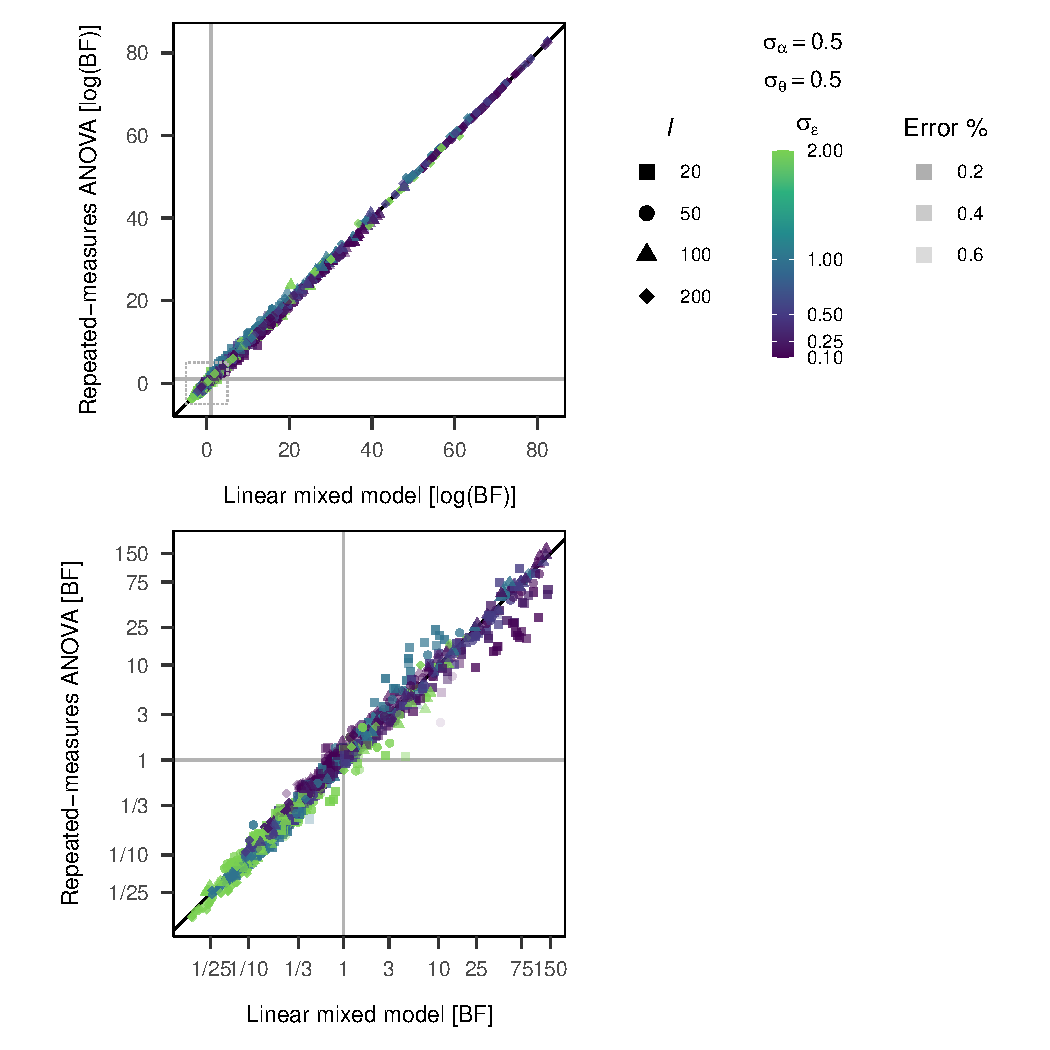
\includegraphics{prior_translation_files/figure-pdf/bias-correction-anova-1.pdf}

Estimated regression coefficients

(\#tab:bias-correction-anova-coef)

\emph{Results for regression of \(\log \mathrm{BF}\) from linear mixed
models on \(\log \mathrm{BF}\) from repeated-measures ANOVAs.}

\begin{longtable}[]{@{}lrcrr@{}}
\toprule()
Predictor & \(b\) & 95\% CI & \(t(1793)\) & \(p\) \\
\midrule()
\endhead
\(\sigma_\epsilon\) & -0.871 & {[}-1.042, -0.700{]} & -9.99 &
\textless{} .001 \\
\(\sqrt{\sigma_\epsilon}\) & 0.374 & {[}0.176, 0.571{]} & 3.71 &
\textless{} .001 \\
\(\sqrt{I}\) & 0.017 & {[}0.008, 0.026{]} & 3.79 & \textless{} .001 \\
\(\sigma_\epsilon\) \(\times\) \(\sqrt{I}\) & 0.005 & {[}-0.004,
0.014{]} & 1.04 & .300 \\
\(\log \mathrm{BF}\) \(\times\) \(\sigma_\epsilon^2\) & -0.316 &
{[}-0.325, -0.307{]} & -68.01 & \textless{} .001 \\
\(\log \mathrm{BF}\) \(\times\) \(\log I\) & 0.003 & {[}0.003, 0.004{]}
& 19.74 & \textless{} .001 \\
\(\log \mathrm{BF}\) \(\times\) \(\sigma_\epsilon^2\) \(\times\)
\(\log I\) & 0.049 & {[}0.047, 0.051{]} & 53.89 & \textless{} .001 \\
\bottomrule()
\end{longtable}

\hypertarget{refs}{}
\begin{CSLReferences}{1}{0}
\leavevmode\vadjust pre{\hypertarget{ref-rouder2012}{}}%
Rouder, Jeffrey N., Richard D. Morey, Paul L. Speckman, and Jordan M.
Province. 2012. {``Default Bayes Factors for ANOVA Designs.''}
\emph{Journal of Mathematical Psychology} 56 (5): 356--74.
\url{https://doi.org/10.1016/j.jmp.2012.08.001}.

\leavevmode\vadjust pre{\hypertarget{ref-vandoorn2021}{}}%
van Doorn, Johnny, Frederik Aust, Julia M. Haaf, Angelika M. Stefan, and
Eric-Jan Wagenmakers. 2021. {``Bayes Factors for Mixed Models.''}
\emph{Computational Brain \& Behavior}.
\url{https://doi.org/10.1007/s42113-021-00113-2}.

\end{CSLReferences}



\end{document}
